\begin{usecase}{07}{Gestione del regolatore semaforico}
\usecaseprimaryactors{Utente autenticato}
\usecasepre{L'utente sta visionando il dettaglio del regolatore semaforico selezionato dalla lista.}
\usecasedesc{L'utente può gestire il funzionamento del regolatore semaforico.}
\usecasepost{L'utente può gestire il funzionamento del regolatore semaforico.}
\label{uc:UC07}
\end{usecase}

\begin{figure}[!h] 
    \centering 
    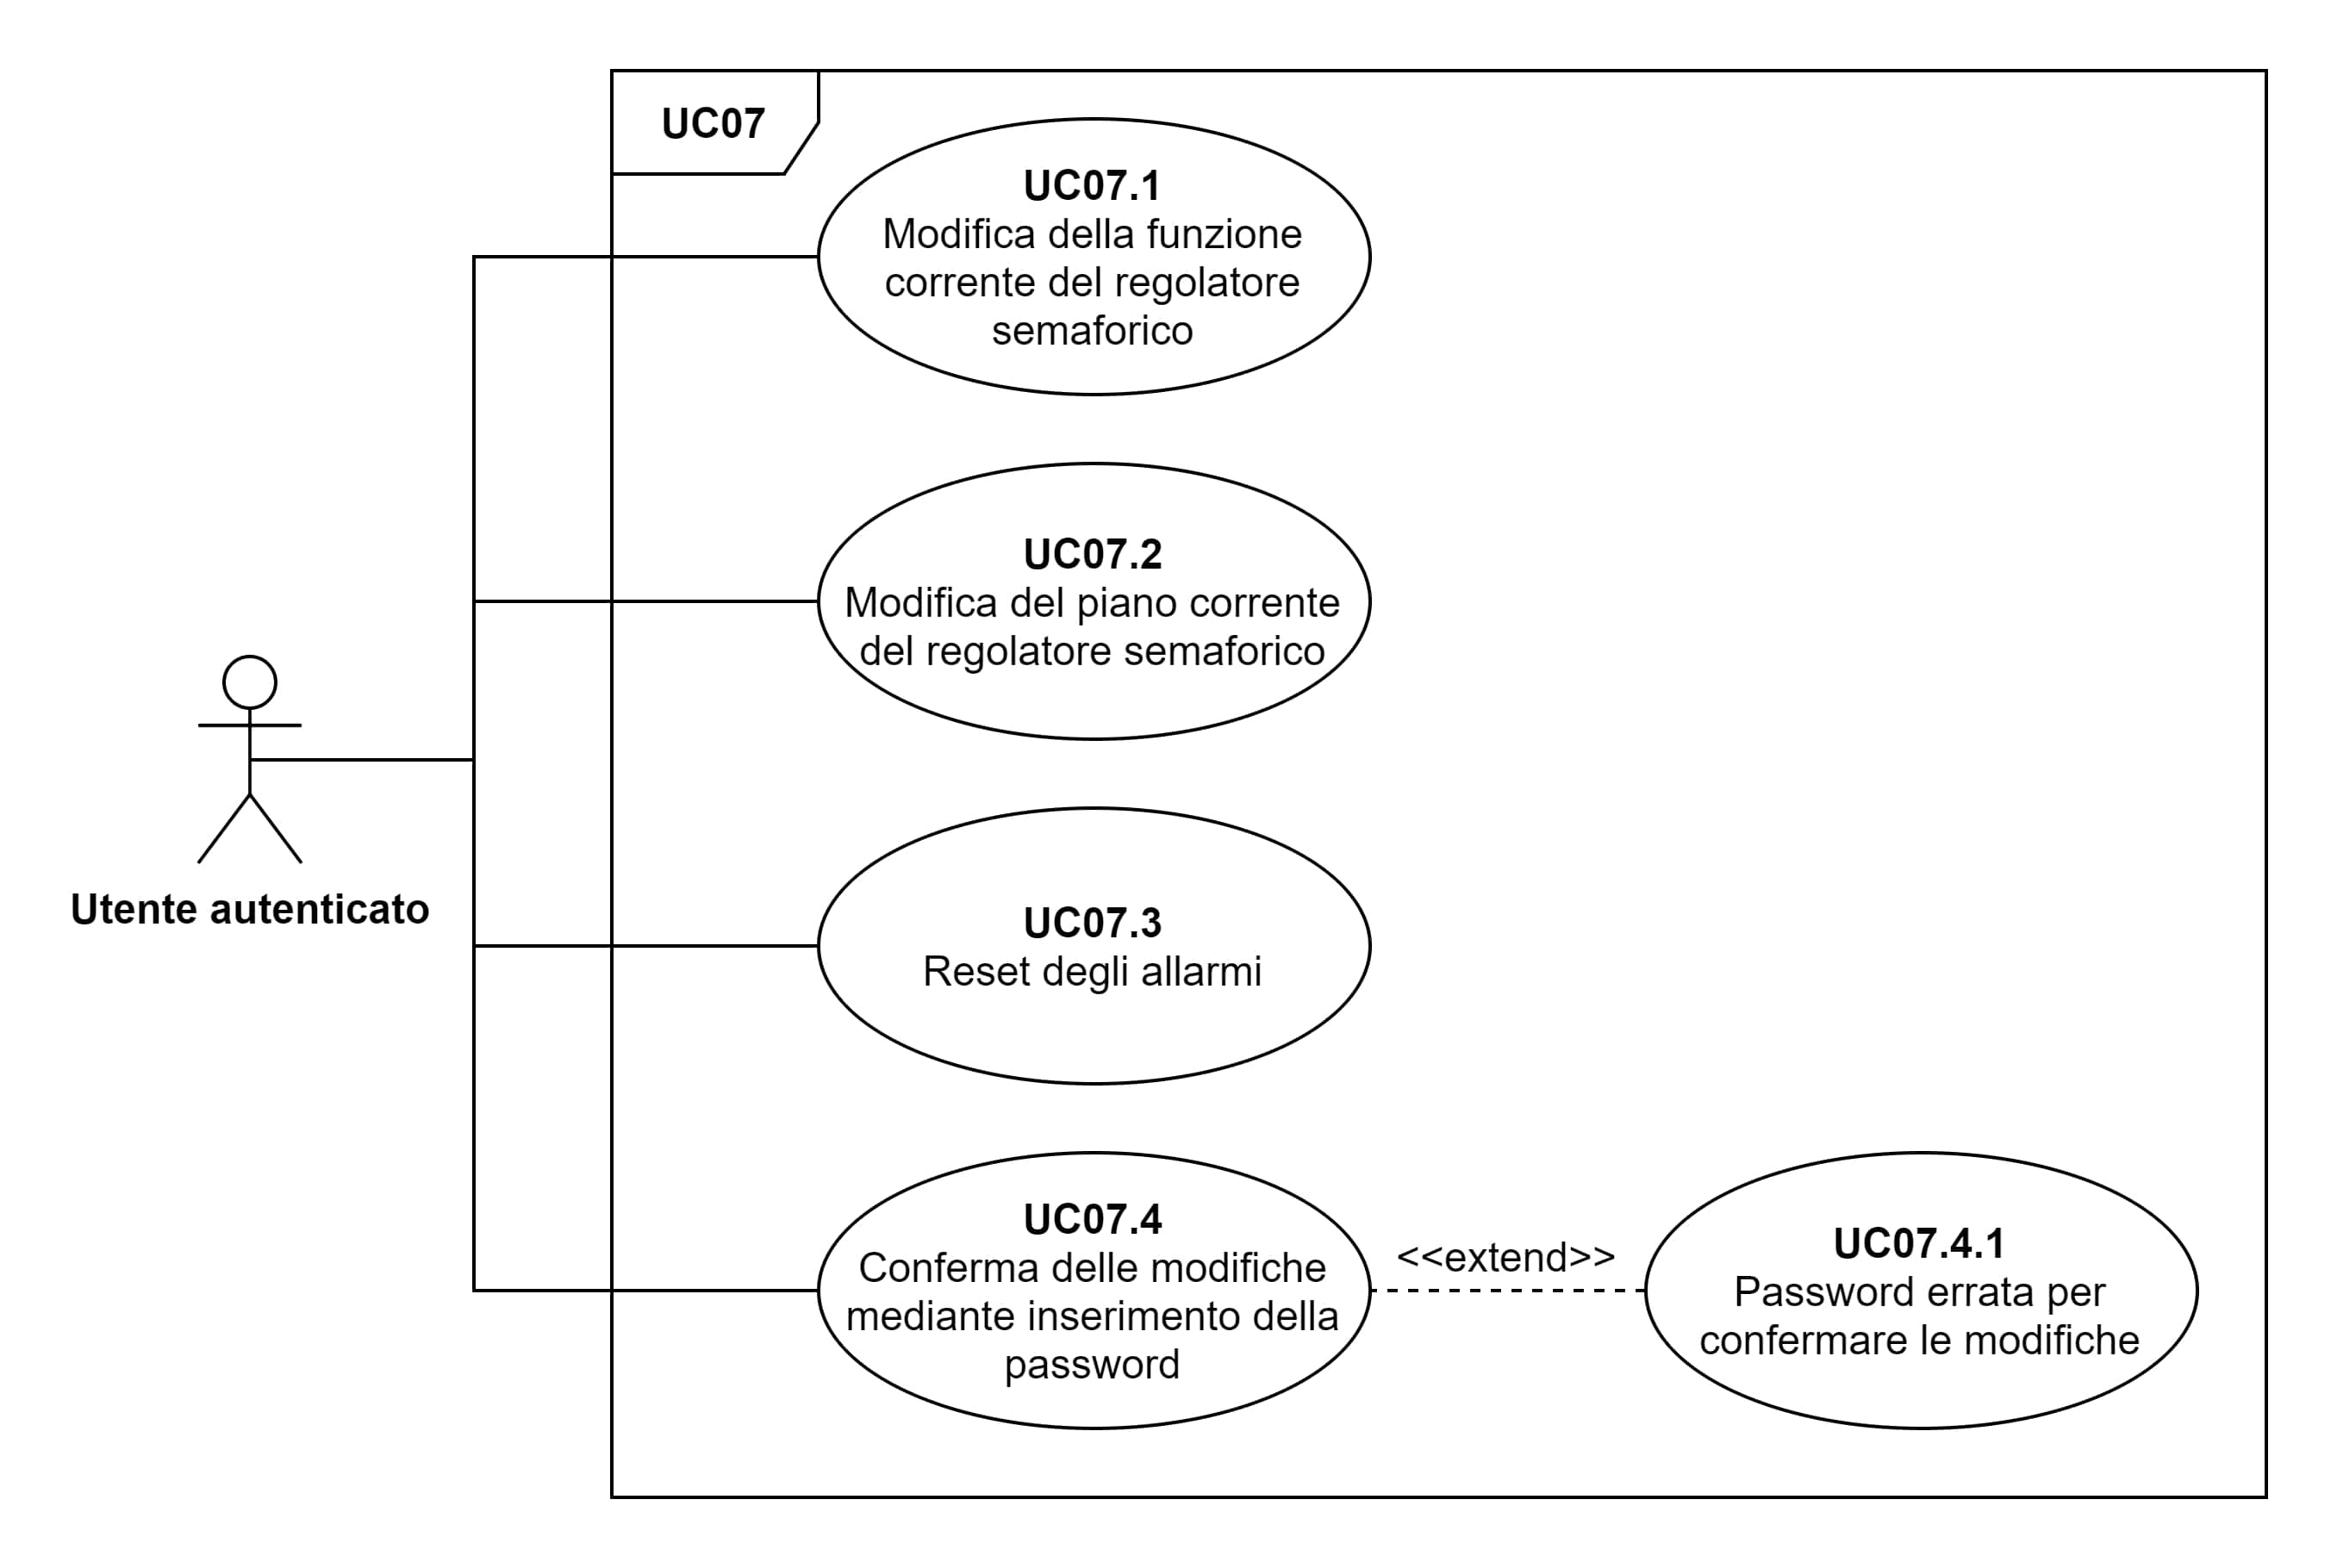
\includegraphics[width=1.0\columnwidth]{appendice-A/uc07} 
    \caption{SMacs - Sotto-casi d'uso di UC07 - Gestione del regolatore semaforico}
\end{figure}

\begin{usecase}{07.1}{Modifica della funzione corrente del regolatore semaforico}
\usecaseprimaryactors{Utente autenticato}
\usecasepre{L'utente ha a disposizione le funzionalità di gestione del regolatore semaforico.}
\usecasedesc{L'utente ha selezionato la funzionalità di modifica e ha aggiornato la funzione corrente del regolatore semaforico.}
\usecasepost{L'utente ha selezionato la funzionalità di modifica e ha aggiornato la funzione corrente del regolatore semaforico.}
\label{uc:UC07-1}
\end{usecase}

\begin{usecase}{07.2}{Modifica del piano corrente del regolatore semaforico}
\usecaseprimaryactors{Utente autenticato}
\usecasepre{L'utente ha a disposizione le funzionalità di gestione del regolatore semaforico.}
\usecasedesc{L'utente ha selezionato la funzionalità di modifica e ha aggiornato il piano corrente del regolatore semaforico.}
\usecasepost{L'utente ha selezionato la funzionalità di modifica e ha aggiornato il piano corrente del regolatore semaforico.}
\label{uc:UC07-2}
\end{usecase}

\begin{usecase}{07.3}{Reset degli allarmi}
\usecaseprimaryactors{Utente autenticato}
\usecasepre{L'utente ha a disposizione le funzionalità di gestione del regolatore semaforico.}
\usecasedesc{L'utente ha selezionato la funzionalità di reset e ha resettato gli allarmi relativi al regolatore semaforico attualmente registrati per il dispositivo.}
\usecasepost{L'utente ha selezionato la funzionalità di reset e ha resettato gli allarmi relativi al regolatore semaforico attualmente registrati per il dispositivo.}
\label{uc:UC07-3}
\end{usecase}

\begin{usecase}{07.4}{Conferma delle modifiche mediante inserimento della password}
\usecaseprimaryactors{Utente autenticato}
\usecasepre{L'utente ha modificato un'impostazione del regolatore semaforico.}
\usecasedesc{L'utente ha modificato un dato di funzionamento del regolatore semaforico e per confermarlo deve inserire la propria password.}
\usecasepost{L'utente ha modificato un dato di funzionamento del regolatore semaforico e per confermarlo ha inserito la propria password.}
\usecaseext{UC07.4.1}
\label{uc:UC07-4}
\end{usecase}

\begin{usecase}{07.4.1}{Password errata per confermare le modifiche}
\usecaseprimaryactors{Utente autenticato}
\usecasepre{L'utente ha inserito la propria password per confermare le modifiche.}
\usecasedesc{L'utente ha inserito una password errata, la modifica non viene confermata e viene avvisato con un messaggio di errore.}
\usecasepost{L'utente ha inserito una password errata, la modifica non viene confermata e viene avvisato con un messaggio di errore.}
\label{uc:UC07-4-1}
\end{usecase}